% ============================================================================
%  Section: Phase Composition and Module Overhead Analysis
%
%  Updated to reflect the persistent backend worker architecture (n=30, 4-inst
%  cross-region deployment). The wall_total denominator is 4,793 ms (was 5,769
%  in the spawn-per-request baseline). Phase percentages, the optimization
%  table, and the summary are all rebuilt against the new measurement.
%
%  Required packages (add to preamble if not already present):
%    \usepackage{graphicx}
%    \usepackage{booktabs}
%
%  Required figure files (place in figures/):
%    figures/fig_phase_composition.pdf
%    figures/fig_salt_comparison.pdf
% ============================================================================

\subsubsection{Phase Composition and Module Overhead Analysis}
\label{sec:phase-module}

This section decomposes the 4.69\,s median end-to-end latency
(\S\ref{sec:e2e-timing}) into per-phase contributions, identifies the
dominant overhead, and quantifies the engineering optimization headroom
that does not require protocol changes.

% ----------------------------------------------------------------------------
% 5.2.1 Phase composition
% ----------------------------------------------------------------------------
\paragraph{Phase Composition}

The wall-clock interval is instrumented at 18 phase boundaries spanning
the browser (11 phases, in \texttt{auth.ts}) and the Node-side backend
served by the persistent worker (7 phases, in \texttt{veramo-to-sui.js}).
Per-phase mean contributions to \texttt{wall\_total} are summarized in
Table~\ref{tab:phase-table} and visualized as a stacked bar in
Figure~\ref{fig:fig_phase_composition}.

\begin{table}[h]
\centering
\small
\caption{Per-phase contribution to \texttt{wall\_total} ($n=30$, in
milliseconds; persistent-worker backend). \emph{Browser misc} aggregates
eight sub-phases of mean $\le 34$\,ms each (epoch fetch, ephemeral key,
randomness, OAuth nonce, JWT parse, nonce verify, save account, bridge
POST). \emph{Node misc} aggregates the four sub-phases of mean
$\le 23$\,ms each (key restore, faucet pre-check, build-and-sign,
signature assembly).}
\label{tab:phase-table}
\begin{tabular}{llrrr}
\toprule
\textbf{Side} & \textbf{Phase} & \textbf{mean (ms)} & \textbf{p50} & \textbf{\% of mean total} \\
\midrule
Browser & ZK proof generation                  & 2{,}586 & 2{,}538 & 54.0\,\% \\
Browser & OAuth round-trip                     &    640 &    630 & 13.4\,\% \\
Browser & Salt fetch (4 inst, parallel)        &    209 &    187 &  4.4\,\% \\
Browser & Browser misc                         &    115 &    103 &  2.4\,\% \\
\addlinespace
Node    & JWK pre-check                        &     13 &     12 &  0.3\,\% \\
Node    & Submit tx + chain finality           &    148 &    109 &  3.1\,\% \\
Node    & Node misc                            &     39 &     39 &  0.8\,\% \\
\addlinespace
\multicolumn{2}{l}{\emph{Unaccounted (page mount, IPC, polling, toast detection)}}
                                               & 1{,}043 & --- & 21.8\,\% \\
\midrule
\multicolumn{2}{l}{\textbf{\texttt{wall\_total}}}
                                               & \textbf{4{,}793} & \textbf{4{,}688} & \textbf{100\,\%} \\
\bottomrule
\end{tabular}
\end{table}

\begin{figure}[h]
\centering
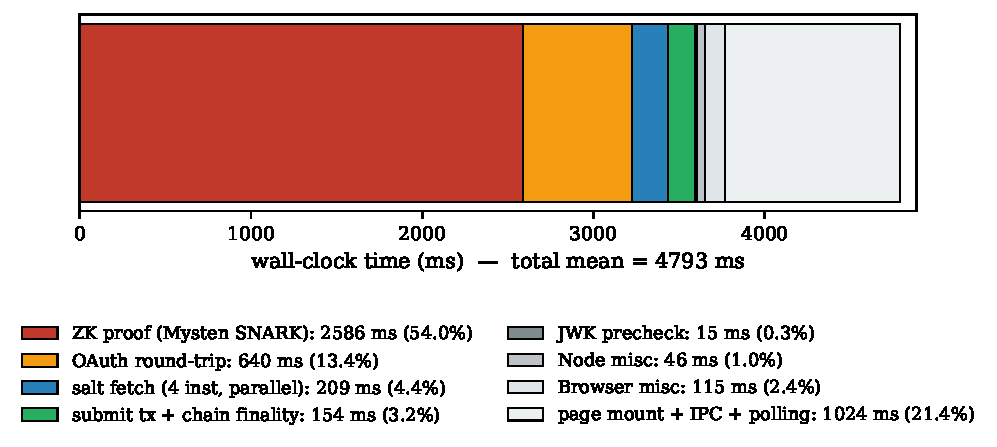
\includegraphics[width=\linewidth]{figures/fig_phase_composition.pdf}
\caption{Stacked decomposition of \texttt{wall\_total} (mean values,
$n = 30$) under the persistent-worker backend. The single largest
contributor is the browser-issued ZK proof request (54.0\,\%); the next
largest is system-layer overhead unaccounted by the 18 phase timers
(21.8\,\%, attributable to page mount, React rendering, IPC, and toast
detection); OAuth contributes 13.4\,\%, while the four-institution
cross-region salt fan-out contributes 4.4\,\%. The two Node-side
on-the-critical-path phases (JWK pre-check and submit + finality)
together account for only 3.4\,\% — a sharp reduction from the
spawn-per-request baseline (8.0\,\%) made possible by the worker's
hot-cache reuse across requests.}
\label{fig:fig_phase_composition}
\end{figure}

\noindent
The most striking feature relative to the spawn-per-request baseline is
the collapse of Node-side overhead. Under spawn mode, JWK pre-check and
submit + chain finality together contributed 460\,ms (8.0\,\%); under
worker mode they contribute only 161\,ms (3.4\,\%) because the worker
keeps the JWKS, Sui balance, and gas-coin metadata caches hot across
trials. The unaccounted system-layer overhead also shrinks from
1{,}664\,ms to 1{,}043\,ms (a 621\,ms reduction) because IPC dispatch
replaces the prior cycle of process spawn, file-based timing
deserialization, and toast-driven polling.

% ----------------------------------------------------------------------------
% 5.2.2 ZK proof generation
% ----------------------------------------------------------------------------
\paragraph{ZK Proof Generation: the Dominant Phase}

Three independent measurements isolate the source of the 2{,}586\,ms ZK
proof phase. First, in-process \texttt{performance.now()} timestamps
around the browser \texttt{fetch} reveal that
\texttt{headerMs} $=$ \texttt{TTFBms} $=$ \texttt{totalMs} $\approx 2{,}586$\,ms,
with \texttt{downloadMs} $\approx 0$ for the 911-byte response: the
client's TCP socket is idle while waiting for the server to emit the
first response byte. Second, an out-of-process Node.js prober that
reuses a stale (\texttt{jwt}, \texttt{randomness}) tuple receives a
\texttt{400 Mismatched JWT Randomness} response in 35--55\,ms (warm
connection) or 119\,ms (cold TLS), proving that Mysten's
request-validation path completes in $<\,$120\,ms before any SNARK
computation. Third, \texttt{curl --trace-time} against the same endpoint
with an empty body returns DNS\,$=$\,1\,ms, TCP connect\,$=$\,2\,ms,
TLS handshake\,$=$\,30\,ms, and TTFB\,$=$\,65\,ms total. Subtracting the
network and request-validate budget gives a server-side Groth16 SNARK
compute time of \(2{,}586 - 65 \approx 2{,}521\)\,ms, accounting for
$97.5\,\%$ of the phase. With this phase now constituting 54.0\,\% of
\texttt{wall\_total} (up from 45.3\,\% in the spawn baseline, simply
because the denominator shrank), the ZK proof is now the unambiguous
dominant phase. It is bound by an external service's compute time, and
is unresponsive to client-side optimizations such as offloading the
request from the browser to a Node.js process or eliminating CORS
preflight.

% ----------------------------------------------------------------------------
% 5.2.3 Cross-region salt fan-out
% ----------------------------------------------------------------------------
\paragraph{Cross-region Salt Fan-out}

We compare three salt-deployment topologies in
Figure~\ref{fig:fig_salt_comparison}: (a) all three institutions
co-located on the browser host (loopback path); (b) all three
institutions deployed in a remote region (\texttt{us-west-1}); and (c)
the four-institution mixed deployment used in the headline measurement.

\begin{figure}[h]
\centering
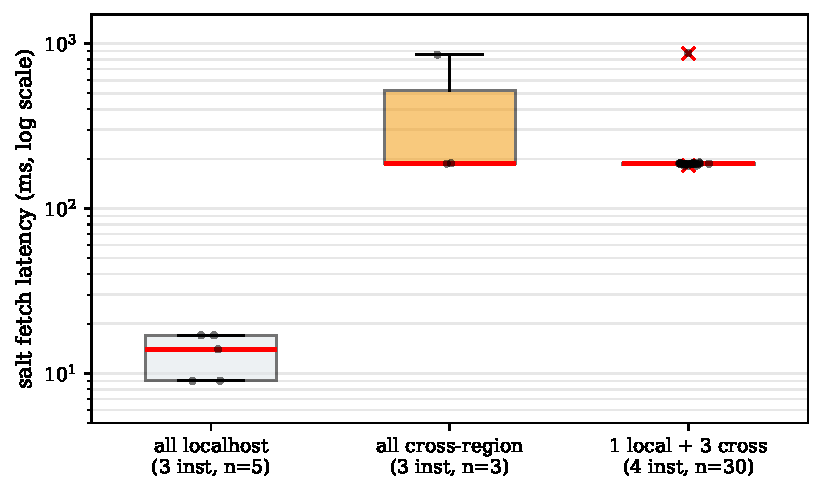
\includegraphics[width=0.6\linewidth]{figures/fig_salt_comparison.pdf}
\caption{Salt fetch latency across deployment topologies (log scale).
Loopback deployment under-reports realistic salt cost by an order of
magnitude (median $14$\,ms); a fully remote deployment varies between
$187$\,ms (warm) and $857$\,ms (cold first connection); the
production-like mixed deployment exhibits a tightly concentrated
warm-state distribution (median $187$\,ms, IQR $\approx 5$\,ms in
Run~2--Run~30), with a single cold-start outlier of $876$\,ms in
Run~1 that lifts the mean to $209$\,ms.}
\label{fig:fig_salt_comparison}
\end{figure}

\noindent
The mixed-deployment salt distribution is governed by
\texttt{Promise.all(...)} fan-out: wall time equals the slowest of four
parallel requests. Empirically the slowest of the three cross-region
hosts dominates and stabilizes at \(\approx 187\)\,ms after the first
trial warms TCP connections; a single Run~1 cold start at 876\,ms
inflates the mean to 209\,ms but the median (187\,ms) remains the
representative steady-state. Two practical implications follow. First,
loopback measurements of salt latency under-report realistic
public-network cost by a factor of $\sim$13$\times$ at the median and
$\sim$50$\times$ in the cold-start case; benchmarks should explicitly
avoid AWS hairpin routing. Second, the salt phase contributes only
4.4\,\% to \texttt{wall\_total} despite running across two AWS regions,
because OAuth (640\,ms) is a longer parallel critical path; salt fits
entirely inside OAuth's shadow.

% ----------------------------------------------------------------------------
% 5.2.4 OAuth and system overhead
% ----------------------------------------------------------------------------
\paragraph{OAuth and System-layer Overhead}

OAuth round-trip is invariant across the three deployments measured
(mean \(\in [639, 688]\)\,ms, sd $\le 45$\,ms), confirming that this
phase is independent of the zkLogin application architecture. The only
levers available are (i) the browser-platform navigate-and-redirect
model itself (replaceable by popup-mode OAuth in which the main window
remains responsive), and (ii) the choice of OAuth provider. The
1{,}043\,ms unaccounted overhead in Table~\ref{tab:phase-table}
consists of page-mount latency, React component re-rendering, the
bridge $\rightarrow$ worker IPC round-trip, and toast detection in the
Playwright observer; this is already 621\,ms below the spawn-mode
baseline because IPC dispatch replaced the file-based timing handoff.
The remaining slice is rooted in the web-based reference implementation
and would shrink substantially in a native client.

% ----------------------------------------------------------------------------
% 5.2.5 Optimization opportunities
% ----------------------------------------------------------------------------
\paragraph{Optimization Opportunities}

Table~\ref{tab:opt} enumerates engineering optimizations identifiable
from the per-phase data. The top section lists optimizations realized
in this study (whose effects are already absorbed in the
\texttt{wall\_total} = 4{,}793\,ms baseline of
Table~\ref{tab:phase-table}); the bottom section lists optimizations
that remain future work.

\begin{table}[h]
\centering
\small
\caption{Latency-reduction opportunities, separated by realization
status. Realized savings are measured against an identically-configured
spawn-per-request baseline (independent $n=30$ run). Future-work savings
are point estimates derived from the per-phase decomposition and the
serial-versus-parallel critical path; values do not carry confidence
intervals at this study's sample size.}
\label{tab:opt}
\begin{tabular}{p{0.42\linewidth}p{0.18\linewidth}rl}
\toprule
\textbf{Optimization} & \textbf{Phase affected} & \textbf{Saving (ms)} & \textbf{Protocol} \\
\midrule
\multicolumn{4}{l}{\emph{Realized in this study (already in the 4{,}793\,ms baseline)}} \\
Persistent backend worker (single Node child, IPC dispatch)
                                            & \texttt{wall\_submit} & \textbf{1{,}023}\,(measured) & none \\
\addlinespace
\multicolumn{4}{l}{\emph{Future work (further headroom from current baseline)}} \\
Self-hosted GPU prover (replaces Mysten dev) & \texttt{prover\_ms} & 1{,}500--2{,}000 & none \\
OAuth and salt parallelization (popup OAuth + non-JWT salt-service auth)
                                             & \texttt{oauth\_rtt} \(\oplus\) \texttt{salt\_ms}
                                                              & $\approx$\,187 & salt-service auth \\
TLS \texttt{preconnect} for prover and Google
                                             & TLS handshake   & $\approx$\,30 & none \\
Pre-OAuth \texttt{Promise.all} (epoch \(\parallel\) eph key \(\parallel\) randomness)
                                             & browser pre-OAuth & $\approx$\,20 & none \\
Post-OAuth \texttt{Promise.all} (salt \(\parallel\) nonce verify)
                                             & browser post-OAuth & $\approx$\,13 & none \\
\midrule
\multicolumn{2}{l}{\textbf{Realized so far}}
                                                                & \textbf{1{,}023} & \\
\multicolumn{2}{l}{\textbf{Further realizable without protocol change}}
                                                                & \textbf{$\approx$\,250} & \\
\multicolumn{2}{l}{\textbf{Theoretical lower bound (incl.\ self-hosted prover)}}
                                                                & \textbf{$\approx$\,2{,}250} & \\
\bottomrule
\end{tabular}
\end{table}

% ----------------------------------------------------------------------------
% 5.2.6 Summary
% ----------------------------------------------------------------------------
\paragraph{Summary}

Three takeaways follow from the module-level decomposition.
\textbf{(i)} The 54.0\,\% contribution of the ZK proof generation phase
is bound by the external prover service's compute time and is not
amenable to client-side optimization. Its share of
\texttt{wall\_total} grew from 45.3\,\% to 54.0\,\% precisely because
client-side overhead has been compressed elsewhere.
\textbf{(ii)} Cross-region multi-institution salt deployment is
performance-feasible at production scale: the four-institution median
contribution is 187\,ms (4.4\,\% of \texttt{wall\_total}) at warm
steady state, demonstrating that distributed salt custodianship does
not degrade end-to-end latency materially under \texttt{Promise.all}
fan-out.
\textbf{(iii)} The persistent backend worker realizes a measured
1{,}023\,ms reduction in \texttt{wall\_total} (\(-17.7\,\%\)), making
it the largest engineering optimization identified outside of the
external SNARK prover. Remaining client-side headroom without protocol
change is approximately 250\,ms across five smaller optimizations.
Achieving substantially better than the current 4{,}793\,ms baseline
would require either replacing the external Mysten prover with a
faster SNARK backend (\(-1500\)~to~\(-2000\)\,ms) or migrating from a
web-based to a native client to reduce the residual 1{,}043\,ms of
system-layer overhead.
